The weak lensing analysis process can be conceptually split into two parts; 1) converting images to catalogs of galaxy shapes and 2) extracting scientific results from shape catalogs. In this section we present a sample image to catalog pipeline. An overview of a weaklensing analysis pipeline is presented in \autoref{fig:pipe}.

\begin{figure}
    \begin{small}
        \begin{center}
            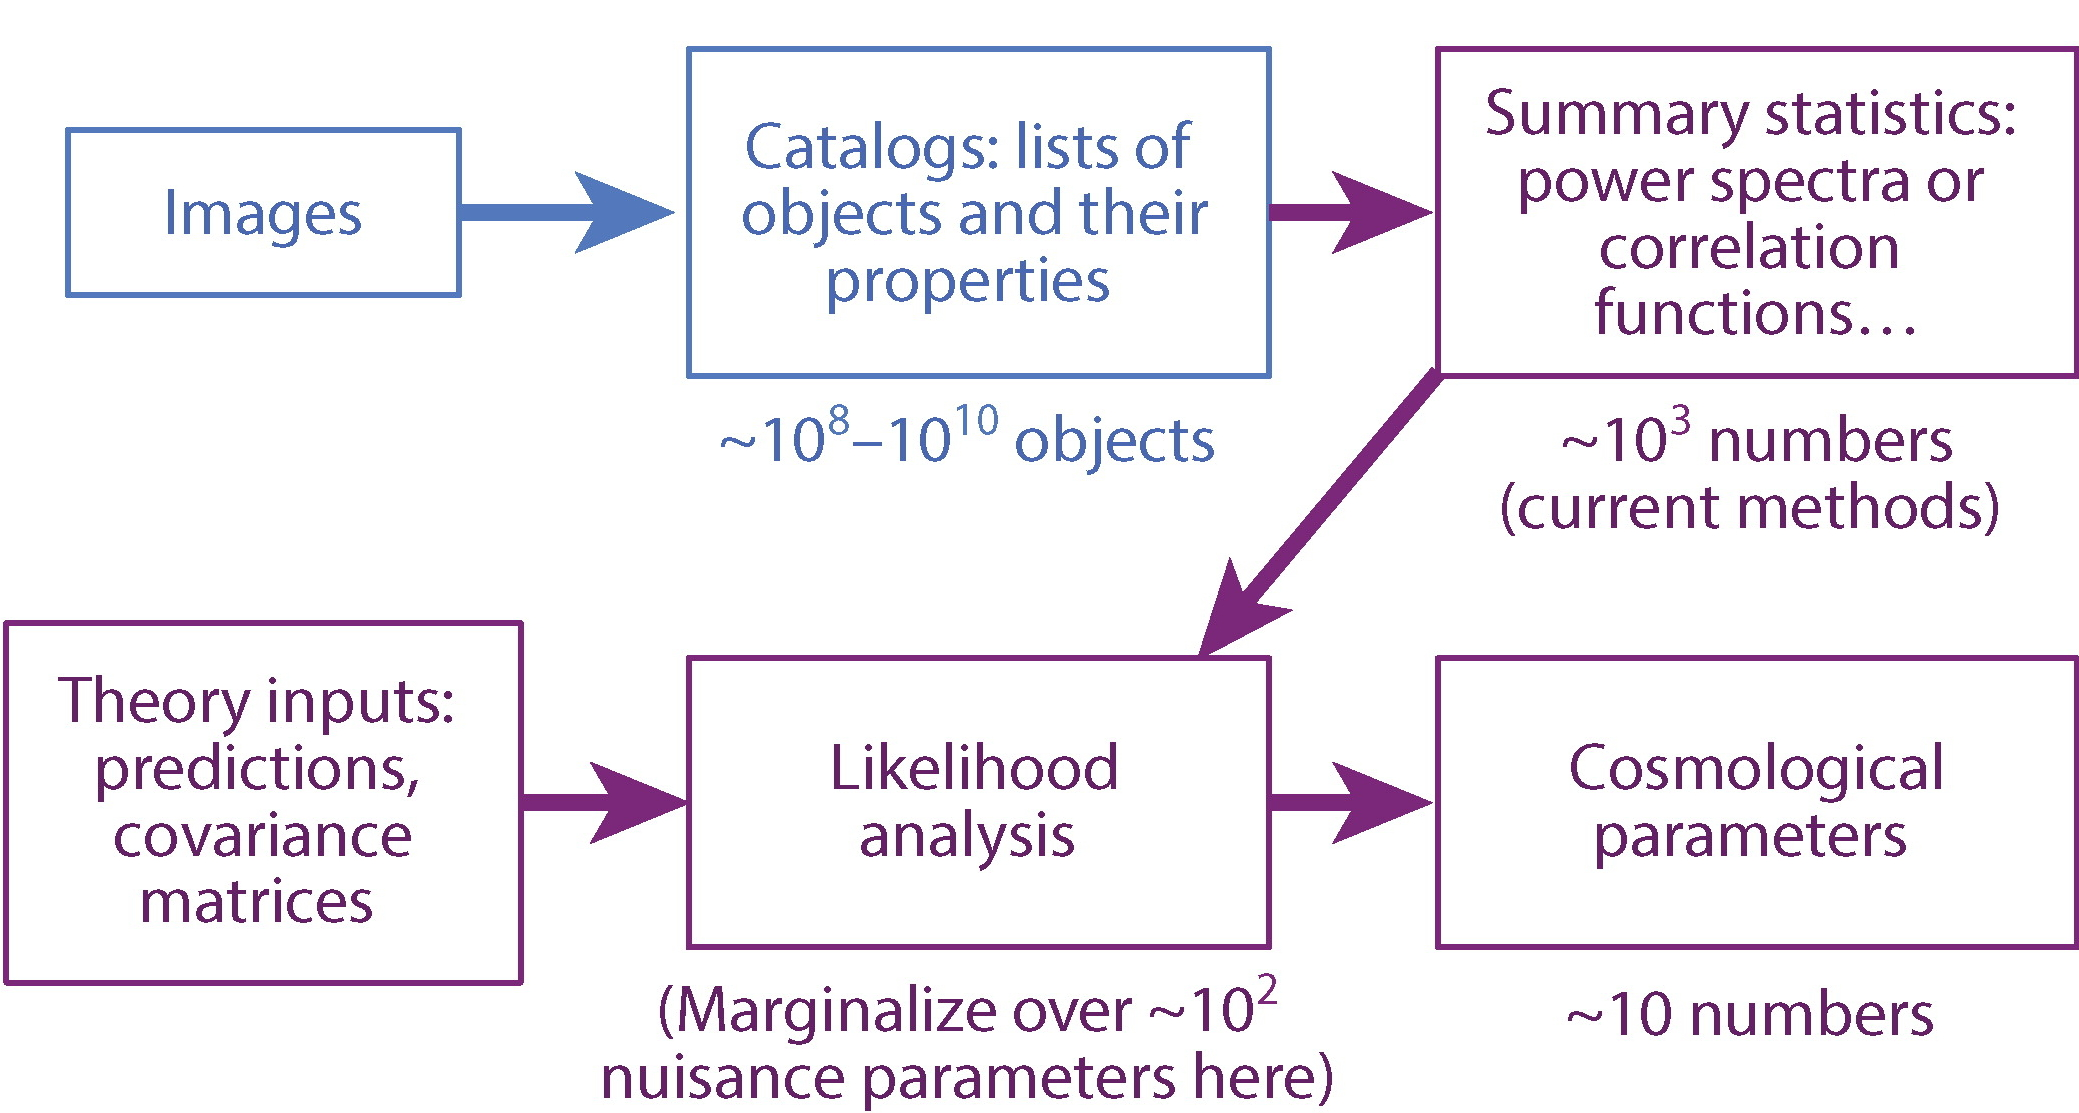
\includegraphics[width=0.95\textwidth]{figs/pipe.jpg}
        \end{center}
        \caption{A generic outline of weak lensing pipeline analysis as presented in \cite{rachel_2018}.}
        \label{fig:pipe}
    \end{small}
\end{figure}


\subsubsection{Object Detection}

The first step in weak lensing analysis is to detect the objects that will be analyzed. In the case of cosmological data the objects of interest are faint distant galaxies. Traditional methods for galaxy detection simply involve the detection of peaks above some detection threshold in a long exposure image. However due to the subtlety of the weak lensing signal the process is more involved. First we must confidently distinguish stars from galaxies, this is a fairly straight forward process that is usually done with photometric data. The next step is to detect galaxies that have blended together in the imaging process, i.e. detections with a double peak feature. Such blended images account for upto 10\% of detections and therefore need to be either deblended or discarded from the data set \cite{rachel_2018,general_2013}.  

\subsubsection{Shape Extraction}
After the galaxies are detected their shapes need to be measured. The accurate measurement of galaxy shape from an image is a rich and complex topic, we will state some results from \cite{massey_2013,general_2013} without derivation. 
Galaxy shapes can also be quantified by computing the moments of the galaxy images.Such methods have been applied to data extensively

\subsubsection{Point Spread Function}

The point spread function (PSF) describes the response of an imaging system to a point source or point object. In practice the surface brightness profile of an object in an image is not the $f_{obs}$ from \autoref{eq:linearizedbright} but is convoloved with some unknown function $PSF(\vec{x})$. Therefore, in order to detect weak lensing signal we must understand and reconstruct our PSF in order to deconvolve it from the image. Deconvolving the PSF is the most important and most difficult step of any weak lensing analysis \cite{Hoekstra:2013gua,rachel_2018}. The PSF has a width which leads to rounder images and typically is anisotropic, which leads to a preferred orientation. The bias is grouped into two kinds: a multiplicative bias $m$ that scales the shear, and an additive bias $c$ that reflects preferred orientations that are introduced. The observed shear and true shear are thus related by

\begin{equation}
    \gamma_{obs} = (1+m) \gamma + c
     \label{eq:shearobs}
\end{equation}



